\section{Schema Decomposition}
\label{sec:sdgd}

\begin{figure}[t]
\centering
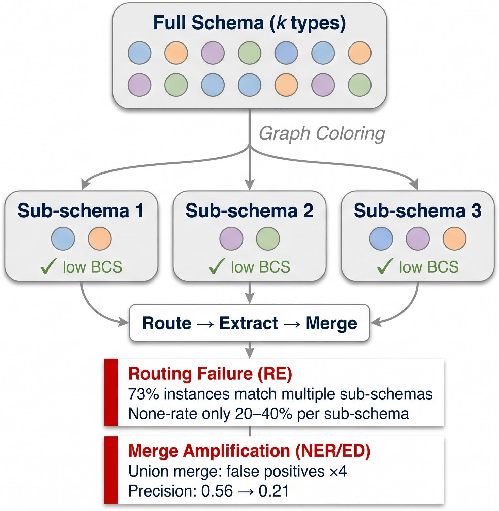
\includegraphics[width=\columnwidth]{../../figures/paper/fig_sdgd_pipeline_compact.pdf}
\caption{Schema decomposition pipeline and failure modes. Graph coloring partitions the schema into low-confusability sub-schemas, but two structural bottlenecks prevent practical gains: \textbf{routing failure} in RE (73.4\% of instances match multiple sub-schemas) and \textbf{merge amplification} in NER/ED (union merge increases false positives ${\sim}4\times$).}
\label{fig:sdgd_pipeline}
\end{figure}

\begin{table}[t]
\centering
\small
\caption{Routing strategy comparison on FewRel 80-relation RE with graph-coloring sub-schema decomposition. Oracle requires gold labels. All practical strategies perform below the single-pass baseline due to constrained decoding: 73.4\% of instances match multiple sub-schemas simultaneously.}
\label{tab:routing_strategies}
\resizebox{\columnwidth}{!}{\begin{tabular}{@{}lrr@{}}
\toprule
\textbf{Strategy} & \textbf{Accuracy} & \textbf{$\Delta$ vs.\ Single-Pass} \\
\midrule
Oracle (gold label) & 72.4\% & +22.0\,pp \\
\midrule
Max-conf (positive only) & 36.5\% & $-$14.0\,pp \\
None-aware & 36.5\% & $-$14.0\,pp \\
Margin (positive only) & 35.9\% & $-$14.5\,pp \\
Max-conf (all) & 27.7\% & $-$22.7\,pp \\
Random & 14.7\% & $-$35.7\,pp \\
\midrule
Single-pass (no decomposition) & 50.4\% & --- \\
\bottomrule
\end{tabular}}
\end{table}

\looseness=-1
A natural intervention is to partition the schema so confusable types never co-occur (Figure~\ref{fig:sdgd_pipeline}). We tested Schema-DAG-Guided Decomposition (SDGD), which applies greedy graph coloring on the SCS graph to assign types to low-confusability batches. While oracle routing recovers accuracy (0.724 vs.\ 0.504 single-pass; Table~\ref{tab:routing_strategies}), all practical routing strategies fall below the single-pass baseline, and NER decomposition amplifies false positives (F1: 0.445$\to$0.251). Merge amplification is the structural bottleneck: union merge increases false positives ${\sim}4\times$ (precision: 0.56$\to$0.21) while voting merge sacrifices recall. Confusability-aware batch composition avoids routing entirely and achieves higher accuracy under oracle assignment (Appendix~\ref{sec:appendix_batch_composition}). Full protocol and routing strategy evaluation in Appendix~\ref{sec:appendix_sdgd}.
